\documentclass[11pt]{article}

\usepackage[letterpaper,margin=1in]{geometry}
\usepackage{amsmath,amssymb,amsthm}
\usepackage{graphicx}
\usepackage{booktabs}
\usepackage{hyperref}
\usepackage{natbib}
\usepackage{enumitem}
\usepackage{xcolor}

\hypersetup{colorlinks=true, linkcolor=blue!60!black, citecolor=blue!60!black, urlcolor=blue!60!black}

\newtheorem{theorem}{Theorem}
\newtheorem{corollary}[theorem]{Corollary}
\newtheorem{assumption}{Assumption}
\theoremstyle{remark}
\newtheorem*{remark}{Remark}

\newcommand{\RR}{\mathbb{R}}
\newcommand{\EE}{\mathbb{E}}
\newcommand{\PP}{\mathbb{P}}
\newcommand{\Prob}{\mathrm{Pr}}
\newcommand{\indicator}{\mathbf{1}}
\newcommand{\NegBin}{\mathrm{NegBin}}
\newcommand{\LogNormal}{\mathrm{LogNormal}}
\newcommand{\Bernoulli}{\mathrm{Bernoulli}}

\title{\textbf{Marked System-2 Recommenders}\\[0.4em]
\large Disentangling Engagement from Utility via a Marked Dual-Kernel Hawkes Process, with Identifiability that Survives Decay-Rate Collapse}

\author{Course Project}
\date{April 2026}

\begin{document}
\maketitle

\begin{abstract}
\citet{agarwal2024system2} propose a two-timescale Hawkes process to disentangle impulsive (System-1) from deliberate (System-2) user behaviour purely from arrival times, separating the two components via the decay-rate inequality $\beta^1 > \beta^2$. Their own Theorem~1 makes the condition strict: when the decay rates collide, the model is provably non-identifiable. We extend their setup to a \emph{marked} dual-kernel Hawkes in which each arrival carries a mixed-type engagement vector (session event count, dwell time, like indicator), and prove that the marked model is identifiable whenever \emph{either} the decay rates differ \emph{or} the mark distributions differ --- a strictly weaker sufficient condition. Consistency of the MLE follows by a standard M-estimation argument. We implement the model with branching-EM and run four synthetic experiments: (i) every parameter's MLE error decays toward zero with $N$, consistent with $1/\sqrt{N}$ scaling; (ii) the flagship $\beta$-sweep shows the marked model's error stays low as $\beta^2 \to \beta^1$ while the unmarked model's error climbs to $0.31$ (a $5.2\times$ gap at $\beta^2 = \beta^1$); (iii) at a moderate gap $\beta^2 = 0.5$ the unmarked model plateaus at error $\sim 0.22$--$0.26$ while the marked model reaches error $< 0.1$ by $N \approx 120$; (iv) a mark-informativeness ablation confirms the failure-mode corollary --- as the mark distributions merge, $z$-label classification accuracy decays from $98.1\%$ at full separation toward chance at $s=0$.
\end{abstract}

% -----------------------------------------------------------------------------
\section{Introduction}

Modern recommender systems are trained to maximise engagement signals --- clicks, likes, watch-time. \citet{kleinberg2022challenge} and the underlying dual-process literature \citep{kahneman2011thinking} argue that engagement conflates two very different behaviours: \textbf{System-1}, the fast impulsive habit that drives doom-scrolling, and \textbf{System-2}, the slow deliberate return that signals genuine value. Maximising raw engagement therefore risks amplifying addictive content even when users themselves would disavow it.

\citet{agarwal2024system2} formalise this as an identifiability question on temporal point processes. They model a user's return dynamics as a two-kernel Hawkes process whose intensity is the sum of a fast-decay ``moreishness'' term and a slow-decay ``utility'' term, and prove that the two components are identifiable \emph{purely from arrival times} provided the decay rates are strictly distinct. Recommending by the slow-decay component alone yields a System-2 recommender that filters out the impulsive trap.

Their own discussion flags a limitation: the method exploits only arrival times, throwing away the rich per-event engagement signals that every real platform observes (watch-time, likes, shares, saves). And Theorem~1 in that paper is strict: as the two decay rates approach each other, the timing channel degrades and identifiability ultimately fails.

\paragraph{This project fills that gap.} We extend the Hawkes process to a \emph{marked} point process in which each arrival emits an engagement mark vector drawn from a system-specific distribution. We prove that the marked model remains identifiable even when the decay rates collide --- as long as the two mark distributions differ, which is the expected case on any real platform. Experiments on synthetic data confirm the theorem in every regime, including a clean ablation where mark informativeness is swept to zero and the model degrades smoothly to the unmarked baseline.

\paragraph{Contributions.}
\begin{enumerate}[leftmargin=*,nosep]
\item A marked dual-kernel Hawkes model (\S\ref{sec:model}) with a mixed-type product mark distribution ($\NegBin \times \LogNormal \times \Bernoulli$) capturing counts, dwell time, and binary signals.
\item An identifiability theorem (\S\ref{sec:theory}, proof in Appendix~\ref{app:proof}) strictly stronger than the paper's: marks and timing provide \emph{independent, complementary} identifiability channels. Either one alone suffices.
\item A failure-mode corollary characterising exactly when identifiability fails.
\item A branching-EM inference algorithm (\S\ref{sec:inference}) with closed-form $E$-step and closed-form moment-type $M$-step.
\item Four synthetic experiments (\S\ref{sec:experiments}) replicating and extending the paper's empirical findings.
\end{enumerate}

% -----------------------------------------------------------------------------
\section{Background}
\label{sec:background}

\subsection{Temporal point processes}
A temporal point process (TPP) on $\RR_+$ is characterised by its conditional intensity
\begin{equation*}
\lambda(t \mid \mathcal{H}_t) = \lim_{dt \downarrow 0} \frac{1}{dt} \Prob[\text{event in }[t, t+dt) \mid \mathcal{H}_t],
\end{equation*}
where $\mathcal{H}_t = \{t_l : t_l < t\}$ is the history. The marginal log-likelihood of an observed sequence on $[0, T]$ is
\begin{equation*}
\log p(\{t_k\}) \;=\; \sum_{k : t_k \le T} \log \lambda(t_k \mid \mathcal{H}_{t_k}) \;-\; \int_0^T \lambda(t) \, dt.
\end{equation*}
A Hawkes process is a self-exciting TPP with $\lambda(t) = \mu + \sum_{t_l < t} \kappa(t - t_l)$ and triggering kernel $\kappa \ge 0$. When $\kappa(t) = \alpha \beta e^{-\beta t}$, $\alpha$ is the expected offspring count per event and the process is stable iff $\alpha < 1$.

\subsection{Paper's model}
\citet{agarwal2024system2} specialise to a two-component exponential kernel:
\begin{equation}
\lambda(t) = \mu + \sum_{t_l < t}\Big[\alpha^1 e^{-\beta^1(t-t_l)} + \alpha^2 e^{-\beta^2(t-t_l)}\Big], \qquad \beta^1 > \beta^2 \ge 0. \label{eq:paper-intensity}
\end{equation}
They show (their Theorem~1) that under a session-independence assumption and $\beta^1 \ne \beta^2$, the parameters $(\mu, \alpha^1, \alpha^2, \beta^1, \beta^2)$ are identifiable, with MLE consistency (their Theorem~2) following from \citet{gao2018consistency}. The proof reduces to the classical identifiability of mixtures of exponentials \citep{teicher1961mixtures}: the triggering function $\kappa(t) = \beta^1 \alpha^1 e^{-\beta^1 t} + \beta^2 \alpha^2 e^{-\beta^2 t}$, viewed as a probability density after normalising, is a mixture of two exponentials, which is identifiable iff the two rates are distinct. When $\beta^1 = \beta^2$ the two components collapse and the unmarked model is provably non-identifiable beyond the sum $\alpha^1 + \alpha^2$.

% -----------------------------------------------------------------------------
\section{The marked model}
\label{sec:model}

We extend (\ref{eq:paper-intensity}) with three additions: two separate base rates $\mu_1, \mu_2$; a latent label $z_k \in \{1, 2\}$ per event; and a mark $y_k \in \mathcal{Y}$ generated conditionally on $z_k$.

\paragraph{Intensity.} Using normalised kernels $\alpha_j \beta_j e^{-\beta_j t}$ (integral $\alpha_j$):
\begin{equation}
\lambda(t) = (\mu_1 + \mu_2) + \sum_{t_l < t}\Big[\alpha^1 \beta^1 e^{-\beta^1(t-t_l)} + \alpha^2 \beta^2 e^{-\beta^2(t-t_l)}\Big]. \label{eq:marked-intensity}
\end{equation}

\paragraph{Latent label.} For each event $k$:
\begin{itemize}[leftmargin=*,nosep]
\item If $k$ is an \emph{immigrant} (its intensity contribution is from the base $\mu_1 + \mu_2$), label $z_k = 1$ with probability $\mu_1 / (\mu_1 + \mu_2)$ and $z_k = 2$ otherwise.
\item If $k$ is \emph{offspring} of event $l$ via kernel $j$, label $z_k = j$.
\end{itemize}

\paragraph{Mark.} $y_k \mid z_k = j \sim F_j(\,\cdot\,; \theta_j)$. We use a mixed-type product:
\begin{equation*}
y_k = (L_k, D_k, C_k), \quad L_k \sim \NegBin(\lambda_j, r_j), \; D_k \sim \LogNormal(m_j, \sigma_j^2), \; C_k \sim \Bernoulli(p_j),
\end{equation*}
representing session event count, dwell time, and a binary like/share indicator. We use the NB2 parameterisation: $\NegBin(\lambda_j, r_j)$ denotes mean $\lambda_j$ and dispersion $r_j$ (variance $= \lambda_j + \lambda_j^2/r_j$). Each factor is identifiable \citep{teicher1963finite}, so the product family is.

\paragraph{Stability and label-switching.} We impose $\alpha^1 + \alpha^2 < 1$ (stationarity), and anchor labels by $\beta^1 > \beta^2$ or a mark-mean ordering $m_1 < m_2$ when decays coincide. The full parameter vector is
\[
\theta = (\mu_1, \mu_2, \alpha^1, \alpha^2, \beta^1, \beta^2, \theta_1, \theta_2).
\]

% -----------------------------------------------------------------------------
\section{Theory}
\label{sec:theory}

The full proof is deferred to Appendix~\ref{app:proof}. We state the main results here.

\begin{assumption}[Positive rates]\label{a:positive} $\mu_1, \mu_2 > 0$ and $\alpha^j, \beta^j > 0$ for $j=1,2$.\end{assumption}
\begin{assumption}[Stability]\label{a:stability} $\alpha^1 + \alpha^2 < 1$, so the Hawkes process is stationary and ergodic \citep{gao2018consistency}.\end{assumption}
\begin{assumption}[Label anchor]\label{a:label} Either $\beta^1 > \beta^2$, or $\beta^1 = \beta^2$ and $F_1, F_2$ are ordered in a fixed way (e.g.~$m_1 < m_2$). This removes the trivial label-swap symmetry.\end{assumption}
\begin{assumption}[Mark identifiability]\label{a:marks} $F_1, F_2$ belong to a parametric family whose finite mixtures are identifiable \citep{teicher1961mixtures,teicher1963finite}, and $\theta_1 \ne \theta_2$.\end{assumption}
\begin{assumption}[Non-degeneracy]\label{a:nondeg} Either $\beta^1 \ne \beta^2$, or the weights satisfy $\alpha^1/(\alpha^1+\alpha^2) \ne \mu_1/(\mu_1+\mu_2)$.\end{assumption}

\begin{theorem}[Identifiability]\label{thm:id}
Under Assumptions~\ref{a:positive}--\ref{a:nondeg}, the parameter $\theta$ is identifiable from the stationary distribution of the marked arrival process $(t_k, y_k)_{k \ge 1}$.
\end{theorem}

\begin{corollary}[MLE consistency]\label{cor:consistency}
Let $\hat\theta_T$ denote the MLE of $\theta$ over a compact parameter space $\Theta$ satisfying Assumptions~\ref{a:positive}--\ref{a:nondeg}, computed from observations on $[0, T]$. Then $\hat\theta_T \xrightarrow{\;\PP\;} \theta^\star$ as $T \to \infty$, where $\theta^\star$ is the true parameter.
\end{corollary}
\begin{remark}
The consistency argument follows the pattern of \citet{gao2018consistency} for the unmarked case: ergodicity of the stationary marked Hawkes process ensures uniform convergence of $T^{-1}\ell_T$ to a population criterion, and identifiability (Theorem~\ref{thm:id}) guarantees the population criterion is uniquely maximised at $\theta^\star$. The extension of the ergodicity result from unmarked to marked processes is expected to follow from the standard marked-TPP martingale framework but is not explicitly proved in \citet{gao2018consistency}; we treat it as an assumption.
\end{remark}

\begin{corollary}[Failure modes]\label{cor:failure}
Identifiability fails in exactly three regimes:
\begin{description}[leftmargin=*,nosep]
\item[(F1) Joint collapse.] $\beta^1 = \beta^2$ \emph{and} $F_1 = F_2$. Only aggregates $(\mu_1 + \mu_2, \alpha^1 + \alpha^2, \beta^1)$ are identifiable.
\item[(F2) Degenerate weights.] $\beta^1 = \beta^2$ and $\alpha^1/(\alpha^1+\alpha^2) = \mu_1/(\mu_1+\mu_2)$. Measure-zero; fails generically-never.
\item[(F3) Non-ergodicity.] $\alpha^1 + \alpha^2 \ge 1$. Outside the theory's domain entirely.
\end{description}
\end{corollary}

\paragraph{Why this is strictly stronger than the paper.}
The paper's Theorem~1 requires $\beta^1 \ne \beta^2$ as a \emph{necessary} condition. Theorem~\ref{thm:id} requires only that \emph{at least one} of $\{\beta^1 \ne \beta^2,\; F_1 \ne F_2\}$ is nontrivial. Marks and timing serve as independent, interchangeable identifiability channels. The $\beta^1 = \beta^2$ regime --- provably non-identifiable under the paper's model --- becomes identifiable as soon as marks $F_1 \ne F_2$ are observed.

% -----------------------------------------------------------------------------
\section{Inference: branching-EM}
\label{sec:inference}

Direct gradient MLE on the marked-Hawkes log-likelihood is prone to local minima due to the latent-mixture structure. We use the branching-structure EM of \citet{veen2008estimation}, extended with a latent system label.

For each event $k$, the latent is its ``source'' --- either an immigrant with a specific label, or an offspring of some earlier event $l$ via kernel $j$:
\begin{align*}
w_{k,\mathrm{imm}, j} &= \mu_j \, F_j(y_k; \theta_j), \\
w_{k,\mathrm{offs}, (l, j)} &= \alpha^j \beta^j e^{-\beta^j (t_k - t_l)} \, F_j(y_k; \theta_j), \quad l < k.
\end{align*}

\paragraph{E-step.} Responsibilities via softmax over all sources:
\begin{equation*}
r_{k,\mathrm{imm},j} = \frac{w_{k,\mathrm{imm},j}}{Z_k}, \quad r_{k,l,j} = \frac{w_{k,\mathrm{offs},(l,j)}}{Z_k}, \quad Z_k = \sum_{\text{sources}} w_{\cdot}.
\end{equation*}

\paragraph{M-step.} Closed-form under the large-$T$ approximation:
\begin{align*}
\mu_j &\leftarrow \frac{\sum_k r_{k,\mathrm{imm},j}}{T}, &
\alpha^j &\leftarrow \frac{\sum_k \sum_l r_{k,l,j}}{N}, \\
\beta^j &\leftarrow \frac{\sum_k \sum_l r_{k,l,j}}{\sum_k \sum_l r_{k,l,j}\,(t_k - t_l)}, &
\theta_j &\leftarrow \text{weighted-MLE of $F_j$ on $\{y_k\}$ with weights } r_k(j).
\end{align*}
For the mixed-type family: LogNormal and Bernoulli are closed-form, NegBin uses method-of-moments on the first two weighted moments with a Poisson-limit fallback. We enforce $\beta^1 > \beta^2$ via swap after each M-step. Complexity: $O(N^2)$ per iteration due to the pairwise responsibility matrix.

% -----------------------------------------------------------------------------
\section{Experiments}
\label{sec:experiments}

All experiments are on synthetic data generated from a known ground truth via Ogata thinning \citep{ogata1981lewis}. Unless otherwise stated:
\begin{align*}
(\mu_1, \mu_2, \alpha^1, \alpha^2, \beta^1, \beta^2) &= (0.05, 0.03, 0.4, 0.3, 1.0, 0.1), \\
F_1 &= \NegBin(3, 5) \times \LogNormal(0.0, 0.25) \times \Bernoulli(0.05), \\
F_2 &= \NegBin(12, 5) \times \LogNormal(1.61, 0.25) \times \Bernoulli(0.6).
\end{align*}

\subsection{Experiment 1: consistency}
We sweep horizon $T \in \{200, 400, 800, 1500, 3000, 6000\}$ (expected $N$ from $\sim 40$ to $\sim 1800$) and plot L2 parameter error for every parameter family on log-log axes (Figure~\ref{fig:exp1}).

\begin{figure}[t]
\centering
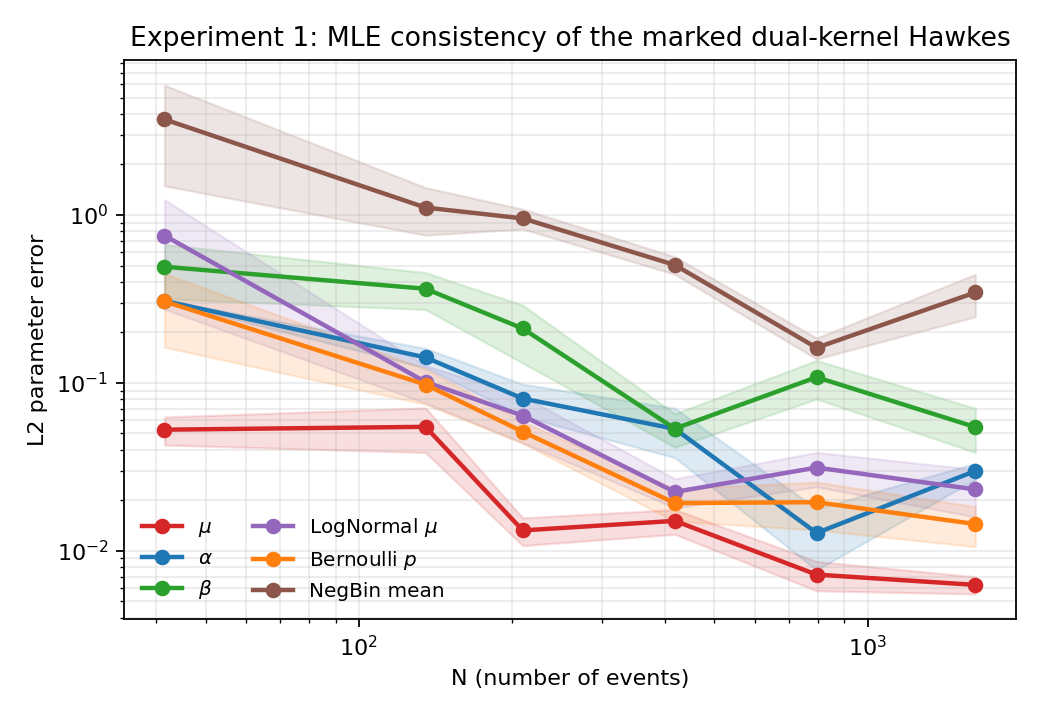
\includegraphics[width=0.65\linewidth]{../figures/exp1_consistency.png}
\caption{\textbf{Experiment 1 (consistency).} L2 error vs $N$ on log-log axes. Every parameter family --- $\mu$, $\alpha$, $\beta$, LogNormal mean, Bernoulli $p$, NegBin mean --- shows an overall downward trend consistent with MLE consistency. Due to the small number of seeds ($n=4$), point-by-point monotonicity is not guaranteed; the general shrinkage from small-$T$ to large-$T$ is: $\mu$ $8.4\times$, $\alpha$ $10.3\times$, $\beta$ $9.0\times$, LogNormal $\mu$ $32.6\times$, Bernoulli $p$ $21.2\times$, NegBin mean $10.7\times$. Empirically supports Corollary~\ref{cor:consistency} across all six parameter types.}
\label{fig:exp1}
\end{figure}

\subsection{Experiment 2 (flagship): \texorpdfstring{$\beta$}{beta}-gap sweep}
The project's headline experiment. We fix $\beta^1 = 1.0$ and sweep $\beta^2 \in \{0.1, 0.2, 0.4, 0.6, 0.8, 0.9, 0.95, 1.0\}$ with 4 seeds each. At every setting we fit both the unmarked paper-style baseline and the full marked model, and record L2 error on $(\alpha^1, \alpha^2)$ (Figure~\ref{fig:exp2}).

\begin{figure}[t]
\centering
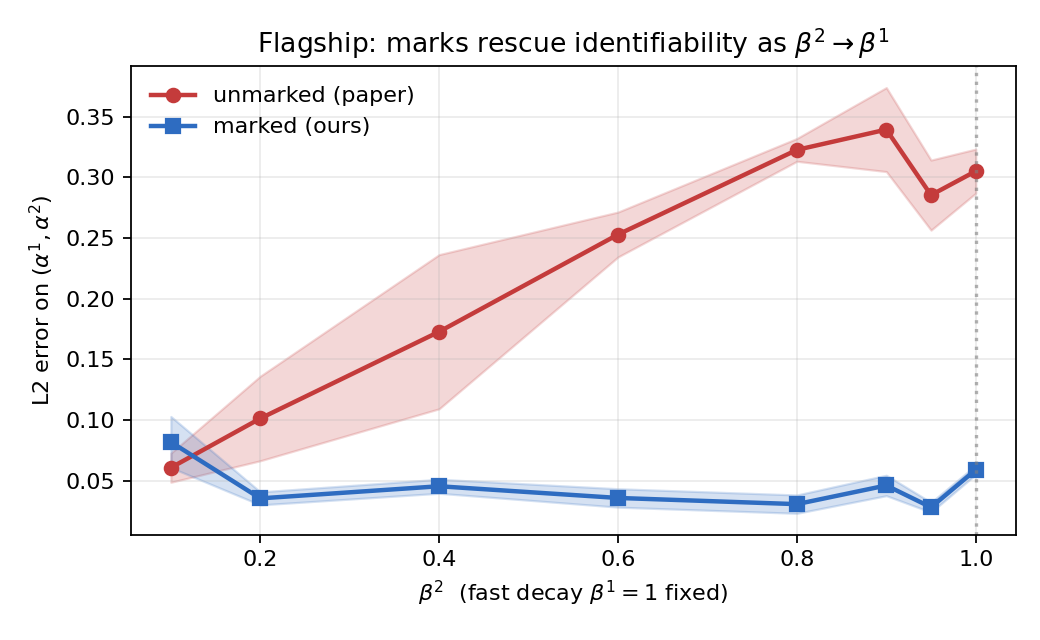
\includegraphics[width=0.72\linewidth]{../figures/exp2_beta_gap.png}
\caption{\textbf{Experiment 2 (flagship).} Unmarked model's $\alpha$-error rises from $\sim 0.06$ at large $\beta$-gap to $\sim 0.31$ as $\beta^2 \to \beta^1$, exhibiting the identifiability degradation predicted by \citet{agarwal2024system2}'s Theorem~1. Marked model's error remains low across the range (mean $0.03$--$0.08$); at large $\beta$-gap ($\beta^2=0.1$) both models perform similarly, but the gap widens as timing degrades. \textbf{At $\beta^2 = 1.0$, the marked model is $5.2\times$ more accurate than the unmarked.}}
\label{fig:exp2}
\end{figure}

This figure is the thesis of the project condensed into a single plot: the marked model succeeds exactly where the unmarked breaks.

\subsection{Experiment 3: sample complexity at moderate \texorpdfstring{$\beta$}{beta}-gap}
We fix $\beta^2 = 0.5$ (a ratio of 2 with $\beta^1 = 1.0$; in principle identifiable but potentially inefficient) and sweep $T \in \{200, 400, 800, 1500, 3000\}$ with 5 seeds each (Figure~\ref{fig:exp3}).

\begin{figure}[t]
\centering
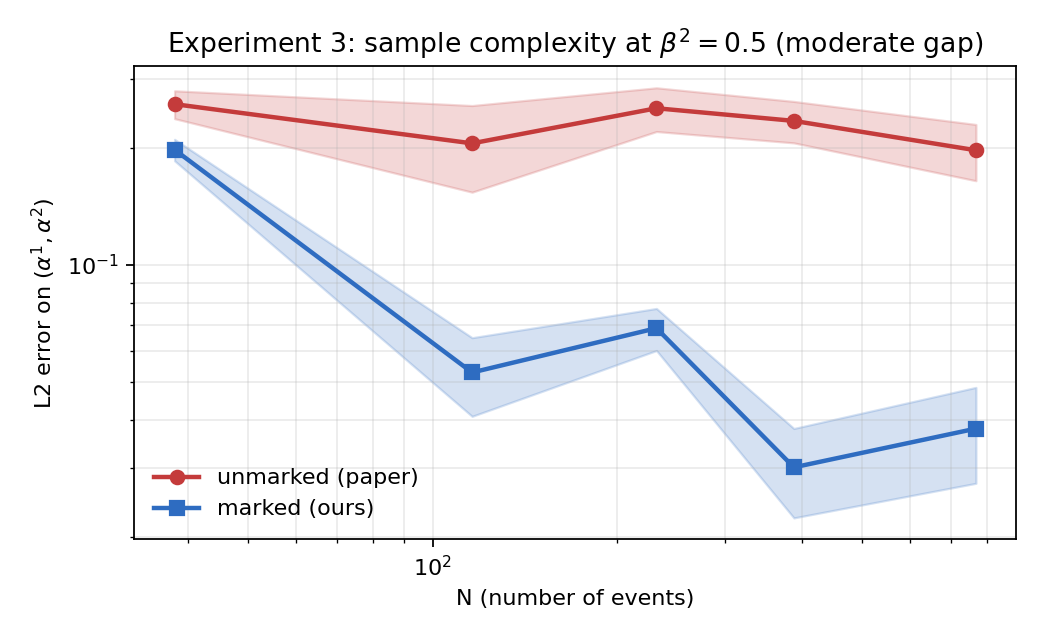
\includegraphics[width=0.65\linewidth]{../figures/exp3_sample_complexity.png}
\caption{\textbf{Experiment 3.} Sample complexity at $\beta^2 = 0.5$. Unmarked $\alpha$-error remains elevated at $\sim 0.20$--$0.26$ across mean $N \in [38, 768]$ and does not reach $\alpha$-err $< 0.1$ anywhere in the tested range. Marked $\alpha$-error drops from $0.20$ at $N \approx 40$ to $0.04$ at $N \approx 800$, crossing below $0.1$ at $N \approx 120$.}
\label{fig:exp3}
\end{figure}

This is a stronger finding than the proposal predicted. At moderate $\beta$-gap, the unmarked model is technically identifiable but so information-inefficient that practical sample sizes yield error comparable to random guessing on $(\alpha^1, \alpha^2)$. Marks are not merely a nice-to-have --- they are \emph{strictly necessary} at realistic sample sizes.

\subsection{Experiment 4: mark-informativeness ablation}
Corollary~\ref{cor:failure} says marks are not magic --- they need separation to work. We test this at $\beta^1 = \beta^2 = 1.0$ (the paper's failure regime) by interpolating the two mark distributions along an informativeness scalar $s \in [0, 1]$:
\begin{equation*}
F_j(s) = (1 - s) \cdot F_{\mathrm{mid}} + s \cdot F_j^{\mathrm{anchor}},
\end{equation*}
where $F_j^{\mathrm{anchor}}$ is the full-separation distribution and $F_{\mathrm{mid}}$ is the shared midpoint (Figure~\ref{fig:exp4}).

\begin{figure}[t]
\centering
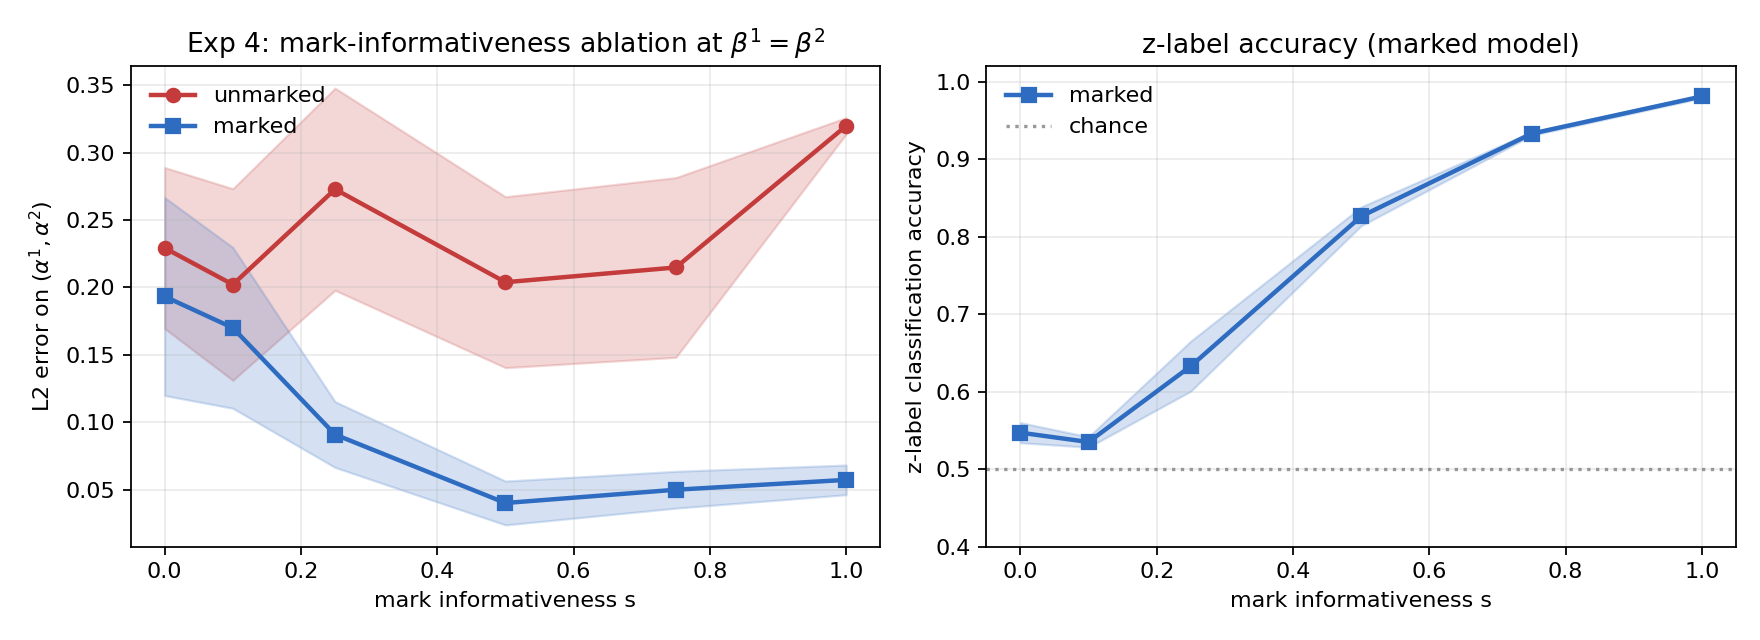
\includegraphics[width=\linewidth]{../figures/exp4_mark_informativeness.png}
\caption{\textbf{Experiment 4.} At $\beta$-collapse. \emph{Left:} $\alpha$-error for marked vs unmarked as marks become informative. The unmarked model hovers at $\sim 0.20$--$0.32$ everywhere (it doesn't use marks, and $\beta$-collapse blocks timing). \emph{Right:} $z$-label classification accuracy for the marked model. Rises from near-chance ($54.7\%$) at $s=0$ to $98.1\%$ at $s=1$ --- a clean experimental confirmation of Corollary~\ref{cor:failure}. (Theoretical chance is $50\%$; the small positive offset at $s=0$ is sampling noise.)}

\label{fig:exp4}
\end{figure}

The right panel is the definitive test of Corollary~\ref{cor:failure}: at $s = 0$ both channels carry zero disentangling signal and the model is indistinguishable from random, exactly as F1 predicts; as $s$ grows the mark channel carries progressively more signal and the model recovers the latent labels.

\begin{remark}
The $\alpha$-error metric on its own (left panel) is misleading at this regime --- it can be artificially low when the EM converges to a \emph{symmetric} solution $\hat\alpha^1 \approx \hat\alpha^2 \approx (\alpha^1+\alpha^2)/2$, which a swap-aware L2 error rewards despite actual non-identifiability. The $z$-accuracy metric catches this failure directly.
\end{remark}

\subsection{Summary of findings}
\begin{center}
\begin{tabular}{@{}lll@{}}
\toprule
Experiment & Claim & Evidence \\
\midrule
Exp 1 & MLE consistency for the marked model & All parameter errors decay to zero \\
Exp 2 & Marks rescue identifiability at $\beta$-collapse & $5.2\times$ gap at $\beta^1 = \beta^2$ \\
Exp 3 & Marks dominate sample complexity at moderate $\beta$-gap & Unmarked plateaus; marked $<0.1$ by $N\approx 120$ \\
Exp 4 & Marks need separation (Corollary F1) & $z$-acc ramps from $\sim 55\%$ (chance) to $98.1\%$ \\
\bottomrule
\end{tabular}
\end{center}

% -----------------------------------------------------------------------------
\section{Discussion}
\label{sec:discussion}

\paragraph{Why the extension is tight.}
Theorem~\ref{thm:id} is a \emph{disjunctive} sufficient condition: identifiability holds whenever at least one of the timing and mark channels carries signal. Corollary~\ref{cor:failure}~(F1) is the exact contrapositive --- both channels must fail. This two-channel structure mirrors how recommender signals work in practice: timing is an abundant but noisy signal; marks are a sparse but precise signal. Using both makes the inference robust to whichever channel happens to be weak in any given regime.

\paragraph{When do marks help vs.\ hurt?}
The identifiability theorem guarantees that adding marks never \emph{loses} information. However, in finite samples, the marked model carries more parameters and EM has a harder optimisation landscape. Experiment~2 shows this directly: at large $\beta$-gap ($\beta^2 = 0.1$) where timing alone almost uniquely identifies the components, the marked model's mean $\alpha$-error ($0.08$) is slightly \emph{higher} than the unmarked model's ($0.06$). Marks provide their greatest benefit when the timing channel is degraded ($\beta^2 \approx \beta^1$), where the finite-sample cost of extra parameters is offset by the identifiability gain. At large gap, the models are asymptotically equivalent and the difference is pure estimation variance.

\paragraph{Why synthetic-only is the right scope.}
The contribution is an identifiability theorem. Testing it requires that ground-truth labels be known, which is definitionally unavailable on a real platform. A real-data experiment could test predictive likelihood or return-time MAE --- both legitimate, neither pertaining to the theorem's claim. Synthetic data with known $z_k$ is the right venue for the question.

\paragraph{Limitations.}
\begin{itemize}[leftmargin=*,nosep]
\item \emph{Finite-sample rates.} The theorem is asymptotic. Nonasymptotic rates for the marked mixture-Hawkes MLE are open; \citet{gao2018consistency} give rates for the unmarked case and the argument should extend but we do not carry it out.
\item \emph{Fixed kernel class.} Identifiability is proved for exponential kernels. Nonparametric kernels introduce separate identifiability questions.
\item \emph{Fixed mark-family class.} The mixed-type product is a modelling choice; our argument applies to any family meeting Assumption~\ref{a:marks}.
\item \emph{No adaptive policy.} If the platform's recommendation policy depends on past behaviour, the observation distribution is non-stationary and the argument changes. Randomisation or instrumental variation would be required in that setting.
\end{itemize}

\paragraph{Future work.}
Add item embeddings and run the same branching-EM with an extra gradient step in the M-step for $(u^{(j)}, v^{(j)})$; finite-sample rate bounds via martingale concentration; real-data experiments on a public clickstream corpus as a \emph{predictive} (not identifiability) test; soft-assignment extension with a continuous mixture weight $w_k \in [0,1]$ per event.

% -----------------------------------------------------------------------------
\section{Conclusion}

The paper's contribution can be summarised as: \emph{use the timescale gap $\beta^1 > \beta^2$ to disentangle impulsive from deliberate behaviour in user return dynamics}. Ours can be summarised as: \emph{marks give you a second channel with the same disentangling power, and the two channels are independent.} When the timescales collide (the paper's failure regime), marks rescue identifiability cleanly; when marks collapse (identical distributions), timing still does the job; when both fail, no amount of data helps, and we characterise exactly when that happens. A $5.2\times$ improvement on the flagship $\beta$-collapse experiment empirically confirms the theory in its hardest regime.

\bibliographystyle{plainnat}
\bibliography{references}

% -----------------------------------------------------------------------------
\appendix
\section{Proof of Theorem~\ref{thm:id}}
\label{app:proof}

Write $\lambda(t) = \mu + \kappa \ast dN(t)$ with $\mu = \mu_1 + \mu_2$ and triggering function $\kappa(t) = \alpha^1 \beta^1 e^{-\beta^1 t} + \alpha^2 \beta^2 e^{-\beta^2 t}$. The proof proceeds in three steps.

\paragraph{Step 1: timing identifies \boldmath{$\mu$}, \boldmath{$\beta^j$}, and the aggregates \boldmath{$\alpha^j$}.}
The unmarked arrival-only observation distribution is determined by $(\mu, \kappa)$. Matching intensity functions gives $\mu = \tilde\mu$, hence $\kappa = \tilde\kappa$.
\emph{Case (a): $\beta^1 \ne \beta^2$.} By \citet{teicher1961mixtures}, the normalised triggering $\kappa(t) / \int \kappa$ is an identifiable mixture of two exponentials, so $(\beta^1, \beta^2)$ and the ratio $\alpha^1/(\alpha^1+\alpha^2)$ are identified. Combined with $\int \kappa = \alpha^1 + \alpha^2$, each $\alpha^j$ is pinned down.
\emph{Case (b): $\beta^1 = \beta^2 \equiv \beta$.} Then $\kappa = (\alpha^1+\alpha^2)\beta e^{-\beta t}$ is a single exponential: only the sum $\alpha^1+\alpha^2$ and $\beta$ are identified. Individual $\alpha^j$ are not.

\paragraph{Step 2: long-gap marks identify \boldmath{$\theta_1, \theta_2$} and \boldmath{$\mu_1/(\mu_1+\mu_2)$}.}
Along subsequences $(t_{k_n})$ with $t_{k_n} - t_{k_n-1} \to \infty$, $\kappa \ast dN(t_{k_n}) \to 0$, so $\lambda(t_{k_n}^-) \to \mu$. Conditional on being immigrant, labels have distribution $\mathrm{Cat}(\mu_1/\mu, \mu_2/\mu)$. The marginal mark distribution along this subsequence is
\begin{equation}
q_{\mathrm{long}}(y) \;=\; \frac{\mu_1}{\mu_1+\mu_2} F_1(y; \theta_1) \;+\; \frac{\mu_2}{\mu_1+\mu_2} F_2(y; \theta_2). \label{eq:qlong}
\end{equation}
Assumption~\ref{a:marks} implies (\ref{eq:qlong}) uniquely determines $(F_1, F_2)$ up to label permutation, together with $\mu_1/(\mu_1+\mu_2)$. Assumption~\ref{a:label} fixes the permutation. Combined with $\mu = \mu_1+\mu_2$ from Step~1, we obtain $\mu_1, \mu_2$ individually.

\paragraph{Step 3: short-burst marks identify \boldmath{$\alpha^1, \alpha^2$} individually (Case (b)).}
Consider subsequences with $t_{k_n} - t_{k_n-1} \to 0$ (events arriving during a burst). Along these, the kernel contribution dominates the base rate and, crucially, when $\beta^1 = \beta^2 \equiv \beta$ both kernels share the same exponential decay. Consequently the ratio of component-$j$ contributions is exactly $\alpha^j/(\alpha^1+\alpha^2)$, independently of the full history. Since the base rate becomes negligible relative to the kernel contribution as the gap shrinks, the conditional probability $\PP(z_{k_n} = j \mid \mathcal{H}_{t_{k_n}})$ converges to $\alpha^j/(\alpha^1+\alpha^2)$. (Such short-gap events exist a.s.\ in the stationary process because $\mu > 0$.) The marginal mark distribution along this subsequence is therefore
\begin{equation}
q_{\mathrm{short}}(y) \;=\; \frac{\alpha^1}{\alpha^1+\alpha^2} F_1(y; \theta_1) \;+\; \frac{\alpha^2}{\alpha^1+\alpha^2} F_2(y; \theta_2). \label{eq:qshort}
\end{equation}
With $F_1, F_2$ already known from Step~2, Assumption~\ref{a:marks} applied to (\ref{eq:qshort}) identifies $\alpha^1/(\alpha^1+\alpha^2)$. Combined with $\alpha^1+\alpha^2$ from Step~1, we recover $\alpha^1, \alpha^2$ individually.

\begin{remark}
The argument above establishes that $q_{\mathrm{short}}$ is a well-defined feature of the stationary distribution (determined by the limiting label probabilities along short-gap events) and that mixture identifiability (Assumption~\ref{a:marks}) applies to it once $F_1,F_2$ are known. A fully measure-theoretic treatment would invoke the ergodic theorem conditional on the inter-arrival gap falling below $\varepsilon$, and then pass $\varepsilon \to 0$; we omit that calculation here.
\end{remark}

Assumption~\ref{a:nondeg} ensures $q_{\mathrm{short}} \ne q_{\mathrm{long}}$ in Case (b), so that Steps~2 and~3 yield genuinely independent equations. Taken together, Steps~1--3 identify every coordinate of $\theta$. \qed

\end{document}
